\documentclass{beamer}

%%%%%%%%%%%%%%%%%%%%---Pacotes Usados---%%%%%%%%%%%%%%%%%% 
\usepackage{xcolor}
\usepackage[latin1]{inputenc}
\usepackage[brazil]{babel}
\usepackage{graphicx}
%\usepackage[utf8]{inputenc}
\usepackage{float}
%http://www.tex.ac.uk/FAQ-RCS.html
\usepackage{svn}
\usepackage{listings}
%%%%%%%%%%%%%%%%%%%%%%---TEMA---%%%%%%%%%%%%%%%%%%%%%
\usetheme{Berlin}
\definecolor{mygrey}{RGB}{66, 66, 66}
\setbeamertemplate{blocks}[rounded][shadow=false]
\addtobeamertemplate{block begin}{\pgfsetfillopacity{0.8}}{\pgfsetfillopacity{1}}
\setbeamercolor{structure}{fg=mygrey}
\setbeamercolor{block title example}{fg=blue!50,bg= blue!10}
\setbeamercolor{block body example}{fg= blue,bg= blue!5}

\lstset{
           language=C++,
           basicstyle=\tiny,
           keywordstyle=\color{blue}\ttfamily,
           stringstyle=\color{red}\ttfamily,
           commentstyle=\color{green}\ttfamily,
           breaklines=true
       }


%%%%%%%%%%%%%%%%%%%%---Informa��es Iniciais---%%%%%%%%%%%%%%%%%% 
\title[Arduino Day]{Instrumenta��o com Arduino:\\ Fun��o Millis() e Buffer Circular}
\author{Gustavo Henrique Leal}
\institute{IDEIA - PUCRS}
\date{\today}
%%%%%%%%%%%%%%%%%%%%---Inicio do Documento---%%%%%%%%%%%%%%%%%% 
\begin{document}

%%%%%%%%%%%%%%%%%%%%%%%%%%%---CAPA---%%%%%%%%%%%%%%%%%% 
\begin{frame}<beamer>
\titlepage
\end{frame}

%%%%%%%%%%%%%%%%%%%%---Introdu��o---%%%%%%%%%%%%%%%%%% 
%\section{Introdu��o}
\begin{frame}{Introdu��o}
  \begin{itemize}
   \item Instrumenta��o no Arduino
  \end{itemize}
\end{frame}


%%%%%%%%%%%%%%%%%%%%---Millis()---%%%%%%%%%%%%%%%%%% 

\section{Millis()}
\subsection{Delay()}
%\usebackgroundtemplate{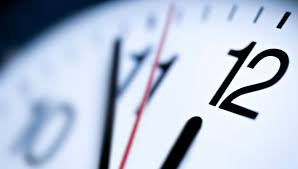
\includegraphics[width=0.5\articlewidth]{images/clock.jpeg}}
%%%%%%%%%%%%%%%%%%%%---Delay()---%%%%%%%%%%%%%%%%%% 
\begin{frame}{Delay()}
         \begin{itemize}
              \item O que �
              \item Como usar
              \item Desvantagens
         \end{itemize}
%         \begin{figure}
%           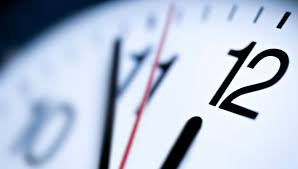
\includegraphics[width=\textwidth]{images/clock.jpeg}
%          \end{figure}
\end{frame}

%\usebackgroundtemplate{\includegraphics[width=\paperwidth]{}}
\begin{frame}[fragile]
  \textbf{Exemplo:}
  \begin{lstlisting}
    void setup() {
      pinMode(7, OUTPUT);
      pinMode(3, OUTPUT);
    }
    
    void loop() {
      digitalWrite(7, HIGH);   // turn the LED on (HIGH is the voltage level)
      delay(1000);                       // wait for a second
      digitalWrite(7, LOW);    // turn the LED off by making the voltage LOW
      delay(1000);                       // wait for a second 
      digitalWrite(3, HIGH);   // turn the LED on (HIGH is the voltage level)
      delay(2000);                       // wait for a second
      digitalWrite(3, LOW);    // turn the LED off by making the voltage LOW
      delay(2000);                       // wait for a second 

    }
  \end{lstlisting}
\end{frame}
%%%%%%%%%%%%%%%%%%%%%%%%%%%%%%%%%%%% ---MIllis()---%%%%%%%%%%%%%%%%%%%%%%%%%
\begin{frame}{Millis}
  \begin{itemize}
    \item Funcionamento;
    \item Vantagens;
    \item Desvantagens.
  \end{itemize}
  
\end{frame}

\begin{frame}[fragile]
  \begin{lstlisting}
    unsigned long lastTimeLed1 = 0;
    unsigned long lastTimeLed2 = 0;
    int ledState = LOW;
    int led2State = LOW;
    void setup() {
      pinMode(3, OUTPUT);
      pinMode(7, OUTPUT); 
    }
    void loop() {
      if( millis() - lastTimeLed1 > 1000){
        lastTimeLed1 = millis();
        
        if(ledState == LOW){
          ledState = HIGH;
        } else {
          ledState = LOW;
        }
        digitalWrite(3, ledState);
      }     
      if( millis() - lastTimeLed2 > 2000){
        lastTimeLed2 = millis();
        if(led2State == LOW){
          led2State = HIGH;
        } else {
          led2State = LOW;
        }
        digitalWrite(7, led2State);
      }
    }
    \end{lstlisting}
\end{frame}


%%%%%%%%%%%%%%%%%%%%---BUFFER CIRCULAR()---%%%%%%%%%%%%%%%%%% 
\section{Buffer circular}
\begin{frame}{Buffer circular}
  \begin{itemize}
     \item O que � um buffer?
     \item LIFO
     \item Aplica��es
     \item Vantagens
  \end{itemize}
\end{frame}
\begin{frame}{Buffer Circular}
    \begin{itemize}
        \item Buffer circular
        \item FIFO
        \item Aplica��es:
          \begin{itemize}
            \item Um processo para outro;
            \item M�ltiplos processos para um;
            \item Um processo para m�ltiplos.
          \end{itemize}
    \end{itemize}
    %%%%%%%%%%%%%%%%%%%%%Adicionar imagem de buffer circular
\end{frame}

\begin{frame}[fragile]
  \textbf{Exemplo: }
  \begin{lstlisting}
    #define BUFFERSIZE 100
    int bufferCircular[BUFFERSIZE];
    int posicao = 0;
    float mediaDoBuffer(){
      unsigned long somatorio = 0;
      for (int i = 0; i < BUFFERSIZE; i++)
      somatorio = somatorio + bufferCircular[i];
      //Serial.println(somatorio);
      return (double) somatorio / BUFFERSIZE;
    }
    void setup(){
      Serial.begin(9600);
      for (int i = 0; i < BUFFERSIZE; i++)
      bufferCircular[i] = 0;
    }
    void loop(){
       bufferCircular[posicao] = analogRead(A5);
      posicao = (posicao + 1) % BUFFERSIZE;
      mediaDoBuffer();
      Serial.println(mediaDoBuffer(), 4);
    }
    
  \end{lstlisting}

\end{frame}

\end{document}
